\documentclass[oneside]{book}
\usepackage{listings}
\usepackage{caption}
\usepackage{subcaption}
\usepackage[all]{xy}
\usepackage{imakeidx}
\makeindex
\usepackage{graphicx}
\usepackage[export]{adjustbox}
\usepackage[spanish]{babel}
\title{Apunte ICPC}

\begin{document}

\lstnewenvironment{codigo}
  {
    \lstset{
        language=C++,
        numbers=left,
        stepnumber=1,
        basicstyle=\footnotesize\ttfamily}
  }
  {
  }


	\maketitle	
	\tableofcontents

	\frontmatter
	\chapter{Notas previas}
	\section{Abreviaciones utilizadas}
\begin{codigo}
typedef long long ll;
//en ciertos casos es necesario cambiar int por ll
typedef vector<int> vi;
typedef vector<vector<int> > vvi;
typedef pair<int,int> ii;
typedef vector<vector<ii> > vvii;		//util para grafos
typedef pair<pair<int,int>,int> iii;
#define mp(x,y) make_pair(x,y)
#define pb(x) push_back(x)
\end{codigo}

	\mainmatter
	\chapter{Estructuras de datos}
	\section{Fenwick Tree}
	\textbf{Nota:} Ambas implementaciones tienen rangos entre 1 a n. \index{Fenwick Tree}
	\subsection{Actualizaciones por rango, consultas puntales }
	\begin{codigo}
struct FenwickTree{
  vi FT;
  FenwickTree(int N){
     FT.resize(N+1,0);
  }

  int query(int i){
     int ans = 0;
     for(;i;i-=i&(-i)) ans += FT[i];
     return ans;
  }

  int query(int i, int j){
     return query(j)-query(i-1);
  }

  void update(int i, int v){
     for(;i<FT.size();i+=i&(-i)) FT[i] += v;
  }

  void update(int i, int j, int v){
     update(i,v); update(j+1,-v);
  }
};

	\end{codigo}
	\pagebreak
	\subsection{Actualizaciones puntuales, consultas por rango}
	La consulta $query(a,b)$ corresponde a la sumatoria de los elementos entre los \'indices $a$ y $b$. \index{RSQ}
	\begin{codigo}
struct FenwickTree {
  vi ft;
  FenwickTree(){}  
  FenwickTree(int n){
    ft.assign(n + 1, 0);
  }

  int query(int b) {
    int sum = 0;
    for (; b; b -= b&(-b)) sum += ft[b];
    return sum;
  }

  int query(int a, int b) { \\RSQ
    return query(b) - (a == 1 ? 0 : query(a - 1));
  }

  void update(int k, int v) {                    // note: n = ft.size() - 1
    for (; k < (int)ft.size(); k += k&(-k)) ft[k] += v;
  }
};
	\end{codigo}
	\section{Union-Find}
	Utilizada para trabajar conjuntos disjuntos. Sirve para encontrar componentes conexas en grafos no dirigidos. \index{Componentes conexas} \index{Conjuntos disjuntos} \index{Particiones}
	\begin{codigo}
class UnionFind {
private:
  vi p, rank, setSize;
  int numSets;
public:
  UnionFind(int N) {
	setSize.assign(N, 1); numSets = N; rank.assign(N, 0);
	p.assign(N, 0); for (int i = 0; i < N; i++) p[i] = i; }
  int findSet(int i) { return (p[i] == i) ? i : (p[i] = findSet(p[i])); }
  bool isSameSet(int i, int j) { return findSet(i) == findSet(j); }
  void unionSet(int i, int j) {  
	if (!isSameSet(i, j)) { numSets--;  
	int x = findSet(i), y = findSet(j);
	// rank is used to keep the tree short
	if (rank[x] > rank[y]) { p[y] = x; setSize[x] += setSize[y]; }
	else               	   { p[x] = y; setSize[y] += setSize[x];
                             if (rank[x] == rank[y]) rank[y]++; } } }
  int numDisjointSets() { return numSets; }
  int sizeOfSet(int i) { return setSize[findSet(i)]; }
};

	\end{codigo}
	
	

	
	\chapter{Grafos}
	\section{Single source shortest path}
	\subsection{Dijkstra}
	Utilizamos la representacion vvii con pares (vecino,peso)
	\begin{codigo}
	asd
	\end{codigo}
	\chapter{Flujo}
	\section{Problemas de asignaci\'on}
	\subsection{Bipartite matching}
	\index{Bipartite matching}
	Tenemos dos conjuntos $A$ y $B$, donde cada elemento de $A$ es compatible con ciertos elementos de $B$. Adem\'as, tenemos la condici\'on de que podemos asociar cada elemento de $A$ con a lo m\'as un solo elemento de $B$. Bipartite matching nos permite saber la cantidad m\'axima de asociaciones posibles.
\begin{figure}[h]
\centering
\begin{subfigure}{.5\textwidth}
\begin{displaymath}
\xymatrix@R-1pc{
&&&*+[o][F-]{B_1} \ar[dddrr]
\\
&&*+[o][F-]{A_1} \ar[ur] \ar[dr]
&*+[o][F-]{B_2} \ar[ddrr]
\\
&&*+[o][F-]{A_2} \ar[r] \ar[dddr] \ar[ur]
&*+[o][F-]{B_3} \ar[drr]
\\
*+[o][F-]{S} \ar[rruu] \ar[rru] \ar[rr] \ar[rrd] \ar[rrdd]
&&*+[o][F-]{A_3} \ar[ur]
&*+[o][F-]{B_4} \ar[rr]
&&*+[o][F-]{T}
\\
&&*+[o][F-]{A_4} \ar[ddr]
&*+[o][F-]{B_5} \ar[urr]
\\
&&*+[o][F-]{A_5} \ar[r] \ar[uur]
&*+[o][F-]{B_6} \ar[uurr]
\\
&&&*+[o][F-]{B_7} \ar[uuurr]
\\
}
\end{displaymath}
\caption*{Modelamiento utilizado. Todas las aristas llevan 1 de flujo.}
\end{subfigure}
\end{figure}
	
	\chapter{Contenido adicional}
	\section{Usar en caso de emergencia}
	\begin{figure}[h]
		\centering
		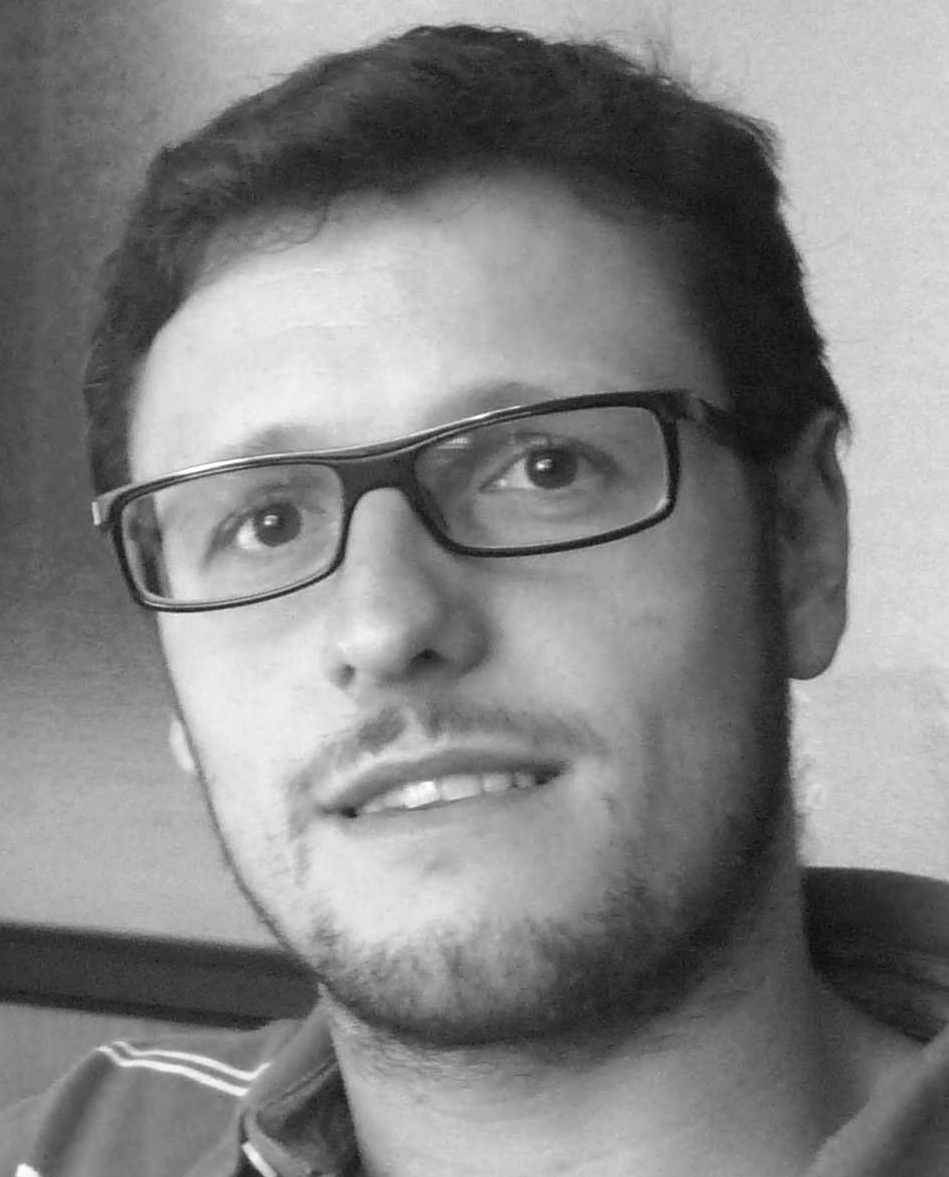
\includegraphics[width=0.7\textwidth]{foto}
		\caption*{GOD BLESS OUR SAVIOUR}
	\end{figure}
	\backmatter
	\printindex
\end{document}